\documentclass{article}
\usepackage{amsmath}
\usepackage{mathrsfs}
\usepackage{amsfonts}
\usepackage{lscape}
\usepackage{graphicx}
\usepackage{caption}
\usepackage{subcaption}
\usepackage{float}
\usepackage{cancel}
%\documentstyle[11pt]{article}
\setlength{\topmargin}{-.5in}
\setlength{\textheight}{9in}
\setlength{\oddsidemargin}{.125in}
\setlength{\textwidth}{6.25in}
\allowdisplaybreaks[1]
\usepackage{indentfirst}

\def\presuper#1#2%
  {\mathop{}%
   \mathopen{\vphantom{#2}}^{#1}%
   \kern-\scriptspace%
   #2}


\begin{document}

\title{CS 5220 HW1: Matrix Multiplication}
\author{Group 23: \\Robert Carson, rac428, Saurabh Netravalkar, sn575, Avi Agarwal, aa2345}
\renewcommand{\today}{17 Sept. 2015}
\maketitle

\section*{Optimization Methods and Methodology:} 

Several different optimization methods were examined during this initial matrix-matrix multiplication assignment including hand tuning the naive matrix-matrix multiplication code, interfacing with a different programming language (Fortran), and using different optimization flags within the compiler.  First, we'll go over the basics of the problem. The numerical problem being examined is a simple matrix-matrix multiplication problem which can be represented as the following in einstein notation  $C_{ik} = A_{ij}B_{jk}$. 
So, it can be seen that a minimum of three loops will be required for this problem in the programming languages used. Although, it should be noted using Fortran 90 standards does allow one to reduce this down to two loops through the use of vectorization. 

\subsection*{Hand Tuning:}

The first set of optimization techniques attempted were to examine the different ways that the basic code could be hand tuned to take advantage of the various ways memory is handled for both the software and the hardware.  Depending on which programming language is used, the memory will be either laid out in row-major order or column-major order. It is because of this that it would be very much desired to have the loops laid out in such a way so that the striding across memory is a minimum. The C language uses a row-major layout default to store 2-D arrays.  So, the loops would be ordered such that from the outermost to innermost loop the following indices are looped through: i, j, k. When this order is used a column of C and B and a single element of A are used in the innermost loop. However in the dgemm functions, all of the matrices used are one dimensional, and hence we are in complete control of the storage layout, and in fact in the dgemm functions in C are storing and accessing the matrices in column major order.  Therefore, the functions written for this assignment will take advantage of the column-major layout, so the loops are ordered as follow to take advantage of this from the outermost to inner most loop: k, j, i. Now the program should only have to take a stride of 1 to access the next element in each array.

While the above will help reduce the memory access time, it does not address the issue of the cache constantly being accessed each loop to refresh the data available which will ultimately lead to the cache becoming thrashed. Therefore, a blocked matrix design is introduced as an attempt to reduce the amount of cache misses while the code is being run. A blocked design can be thought of as the following:

\begin{equation*}
 [C] = [A][B]
 \end{equation*}
 \begin{equation*}
\begin{bmatrix}
C_{11} & \hdots & C_{1N} \\
\vdots & \ddots & \vdots \\
C_{N1} & \hdots & C_{NN}
\end{bmatrix} = \begin{bmatrix}
A_{11} & \hdots & A_{1N} \\
\vdots & \ddots & \vdots \\
A_{N1} & \hdots & A_{NN}
\end{bmatrix} \begin{bmatrix}
B_{11} & \hdots & B_{1N} \\
\vdots & \ddots & \vdots \\
B_{N1} & \hdots & B_{NN}
\end{bmatrix}
\end{equation*}

\noindent where $C_{11}$ is a sub matrix of the entire matrix. The size of the blocks can then be controlled by determining what cache is being targeted. The cpu on the totient server have the following cache sizes: L1 32 KB, L2 256 KB, and L3 15 MB (shared across 6 cores). If the assumption is made that only two block matrices will be needed to be loaded into the cache, than the following "ideal" block sizes can be found for each cache L1  44x44, L2 126x126, and L3 395x395. Though the L3 block size could shrink or expand depending on how much memory is allowed to be allocated between the 6 cores. Since the other block matrix will only be using an element at a time, it should be able to fit into the register.\\

Another method that is being attempted currently is to make a local copy of each array. The reasoning behind this is that for large matrices the memory will contain large strides between each column/row. Therefore even if the block size is small, the values of the block matrix will have to be continuously be fetched from memory. It is because of this that a local copy will want to be made of that array so that all of its memory will be located in a continuous location in memory leading to quicker access in the cache.

\subsection*{Interfacing with different programming languages:}

It is known that C does not have the best built-in support for handling matrix calculations. Therefore, Fortran code is also being written that takes advantage of the above hand tuning options from the above sub-section. Since, it contains better built-in support for handling various different numerical calculations. Several Fortran 90 standards are also being examined to see what effects they have on optimizing the code. For example, the ability to vectorize a variable and perform a vector of dot product calculations is looked at because of the fact that is allows for one to eliminate an entire loop out of the matrix computation. An example of that can be seen in the below code snippet:
\begin{verbatim}

do k = 1,ltb
    do j = 1,lta
        c(:, k) = c(:, k) + a(:, j)*b(j, k)
    end do
end do

instead of:

do k = 1,ltb
    do j = 1,lta
       do i =1,lda
           c(i, k) = c(i, k) + a(i, j)*b(j, k)
       end do
    end do
end do


\end{verbatim}

\subsection*{Compiler Flags:}

The compiler has several flags in it that allow for several different automatic optimizations within the code. Several different compiler flags where used that unrolled certain portions of the loops and vectorized various different parts of the code as well.  Also, the general optimization level 3 flag was used as well that performed a myriad of different optimizations that can be found in the intel compiler site. The following flags were used:

\begin{verbatim}
-O3 -funroll-loops -ftree-vectorize -ipo -xHost -ansi-alias -no-prec-div 
       -axCORE-AVX2  -mtune=core-avx2
\end{verbatim}

The O3 flag tells the optimizer to perform a series of aggressive optimizations that can be generally applied on any machine. The funroll-loops is a GNU compiler option $[1]$ that tells the compiler to unroll the loops that the compiler believes would lead to a speed up. The ftree-vectorize option is another GNU option that performs vectorizations on trees. The ipo flags $[2]$ tells the compiler to do interprocedure optimizations, so this means that the compiler is going to attempt to reduce the amount of time that exists when functions are in different files. The xHost flag $[3]$ applies a high level vectorization to the code. Then the ansi-alias flag $[4]$ tells the compiler that pointers passed into a function do not point to the same location in memory. The restrict keyword in C also tells the compiler this as well. The no-prec-div flag $[5]$ tells the compiler to not follow the IEEE standard for division exactly, and instead it can be a little less precise and speed up the results partially. Finally, the axCORE-AVX2  and mtune$=$core-avx2 $[3]$ flags tell the compiler to take advantage of the fact that our CPU has access to the AVX2 vectorization operations, and therefore we want our code to be tuned to this AVX2 instruction set. 

\section*{Results:}

The different optimizations techniques had a profound effect on influencing efficient the matrix-matrx multiplication could become. In Figure 1, the results from a C code from initially blocking the matrix and using a 512 block size  can be seen. It also did not fully at this point fit the 2 arrays into the L3 because at this point it was wrongly assumed that the L3 cache was 15 MB for only the 2. This code also takes some advantage of ensuring the amount of stride lengths for each matrix is a minimum, but it is still not the most optimal design. The only optimization flag turned on at this point is the O3 flag.

\begin{figure}[H]
  \centering
    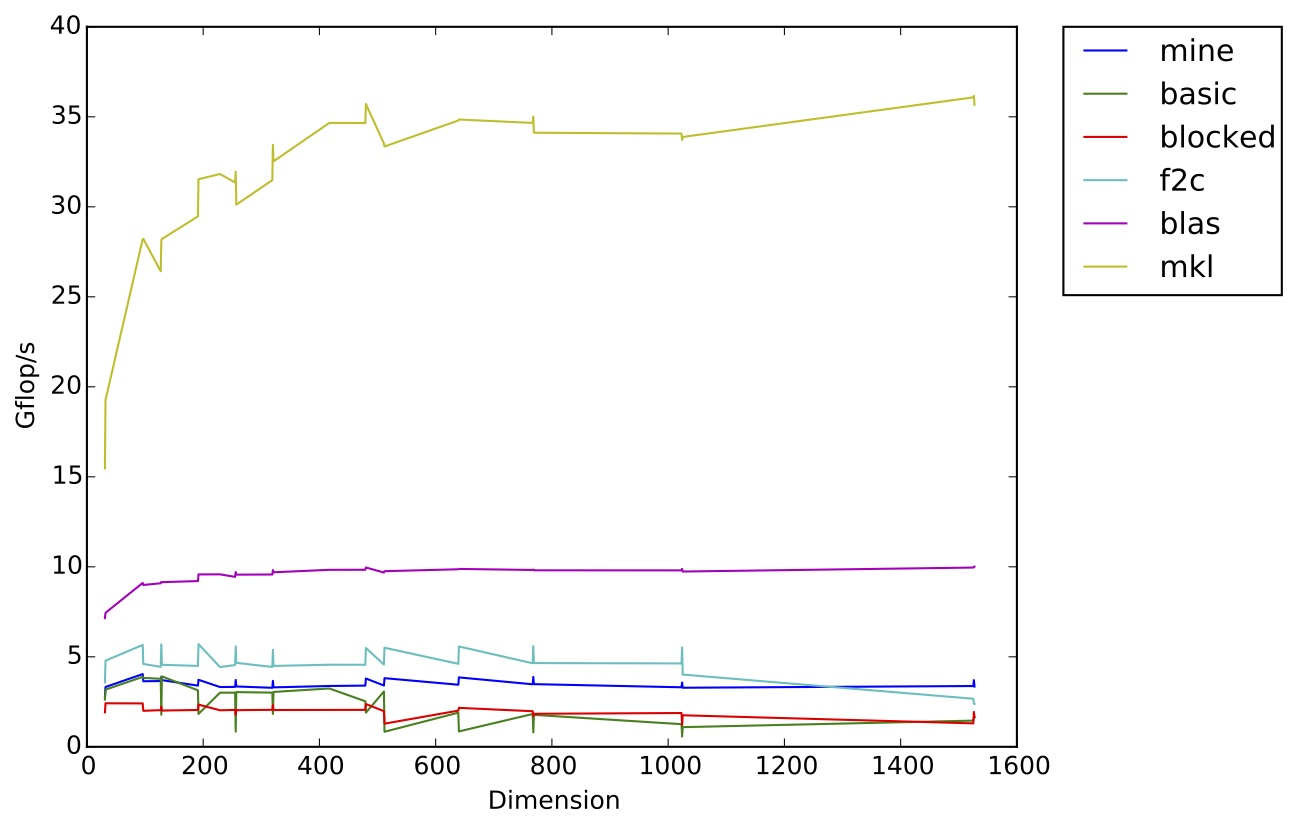
\includegraphics[width=0.8\textwidth]{cblocked_no_opt_flags}
    \caption{Blocked C matrix-matrix multiplication code with a blocked size of 512}
\end{figure}

\noindent It can be seen from Figure 1 that the blocking has helped stabilize the number of flop/s the program is able to do as the dimensions of the inputted matrices increase. Now this same blocking scheme is applied to a Fortran interfaced with C code, and the Fortran scheme is also taking advantage of allowing the strides taken in memory to be a minimum. The results can be found in Figure 2.

\begin{figure}[H]
  \centering
    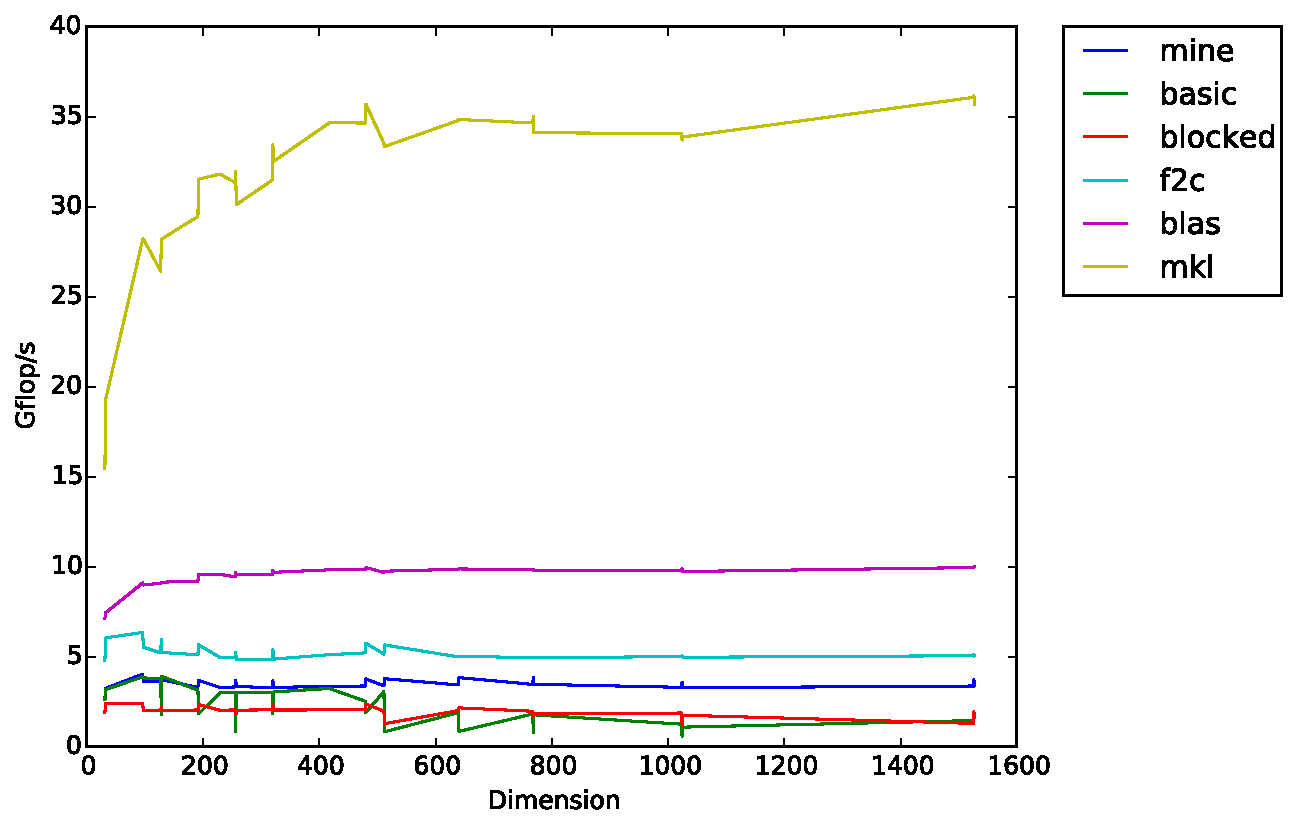
\includegraphics[width=0.8\textwidth]{c_f_blocked_no_opt_flags}
    \caption{Blocked C and Fortran matrix-matrix multiplication code with a blocked size of 512}
\end{figure}

\noindent While these results are an improvement over the naive approaches seen in the basic and blocked approaches, they are still only a fraction of the results obtained from the MKL and OpenBLAS libraries tuned to the server. It should be noted that the OpenBLAS results shown in Figures 1 and 2 are not using the optimized version.  Next, the optimized results that are using the optimization flags mentioned in the Compiler Flags subsection are introduced as well ensuring the block size being used will either fit into the L2 or L3 cache. This code also uses the most optimized form of code that takes advantage of the matrices layout in order to reduce the stride lengths taken. The results shown in Figures 3 use a block size of 380 which is a bit under the L3 cache size in order to accommodate for any other data that might end up being in the cache. The results shown in Figure 4 use a block size of 100 which is just under the L2 cache size for the same reasoning used in the L3 cache results. 

\begin{figure}[H]
  \centering
    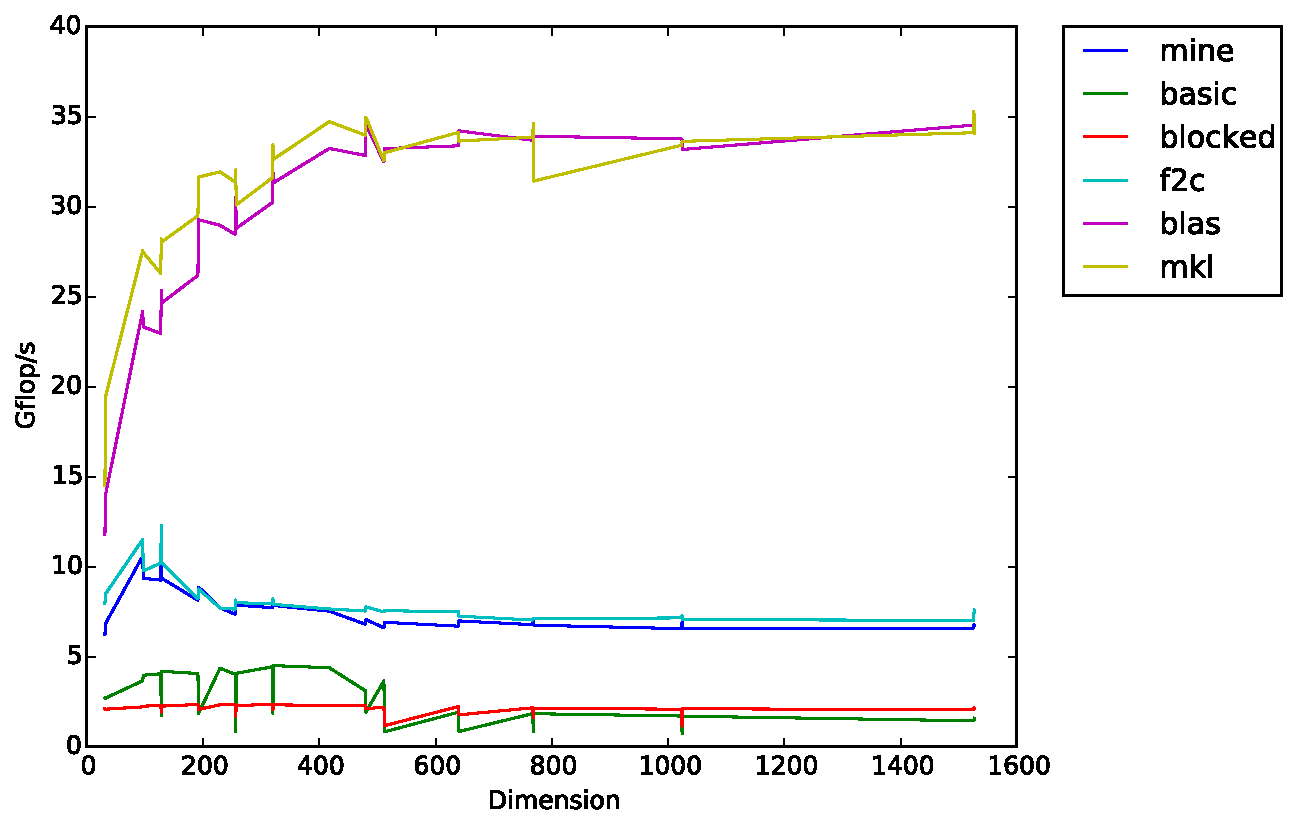
\includegraphics[width=0.8\textwidth]{c_f_blocked_opt_flags_b380}
    \caption{Optimized blocked C and Fortran matrix-matrix multiplication code with a blocked size of 380}
\end{figure}

\begin{figure}[H]
  \centering
    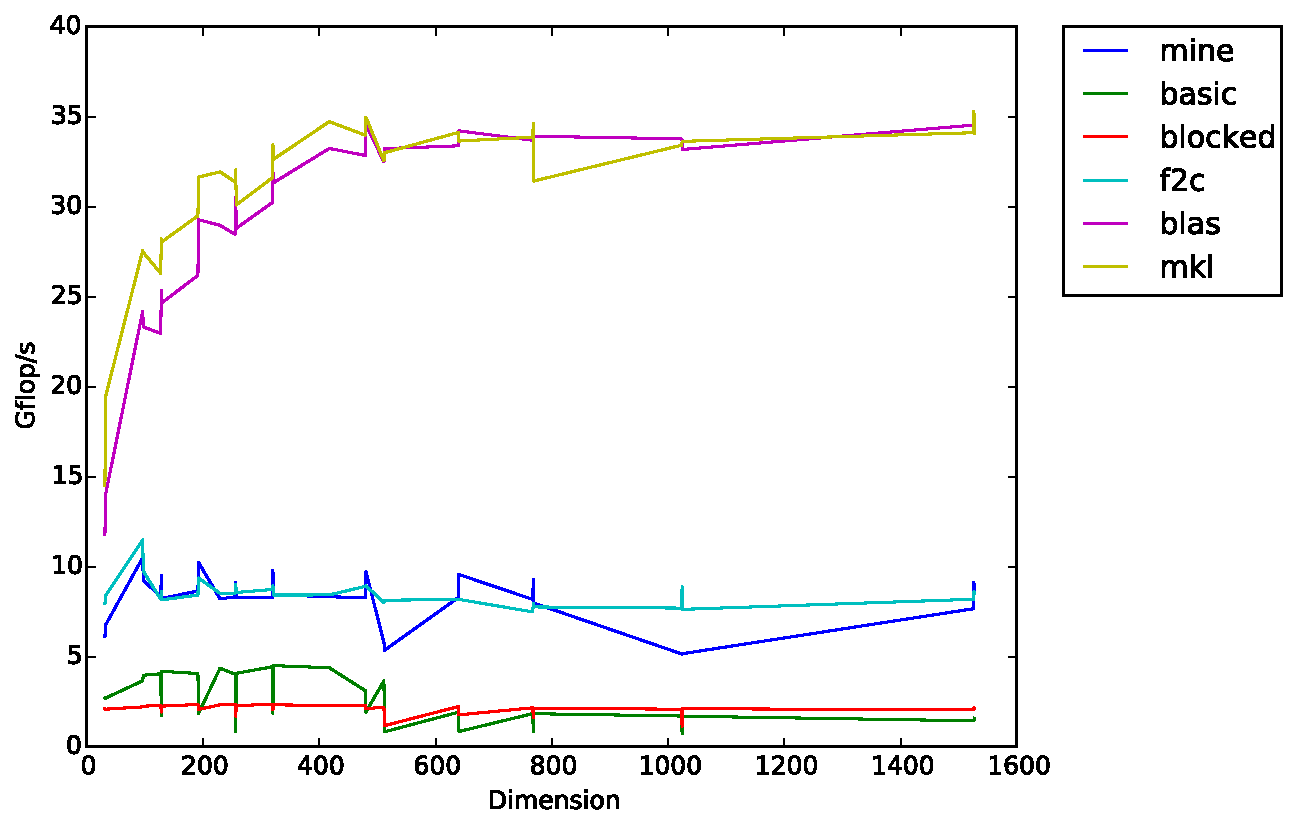
\includegraphics[width=0.8\textwidth]{c_f_blocked_opt_flags_b100}
    \caption{Optimized blocked C and Fortran matrix-matrix multiplication code with a blocked size of 100}
\end{figure}

\noindent  It should be noted that the optimized version of the OpenBLAS was used in the creation of these figures. Finally, these optimization flags were also applied to the naive Fortran code to see what results they have on it, and those can be found in Figure 5.

\begin{figure}[H]
  \centering
    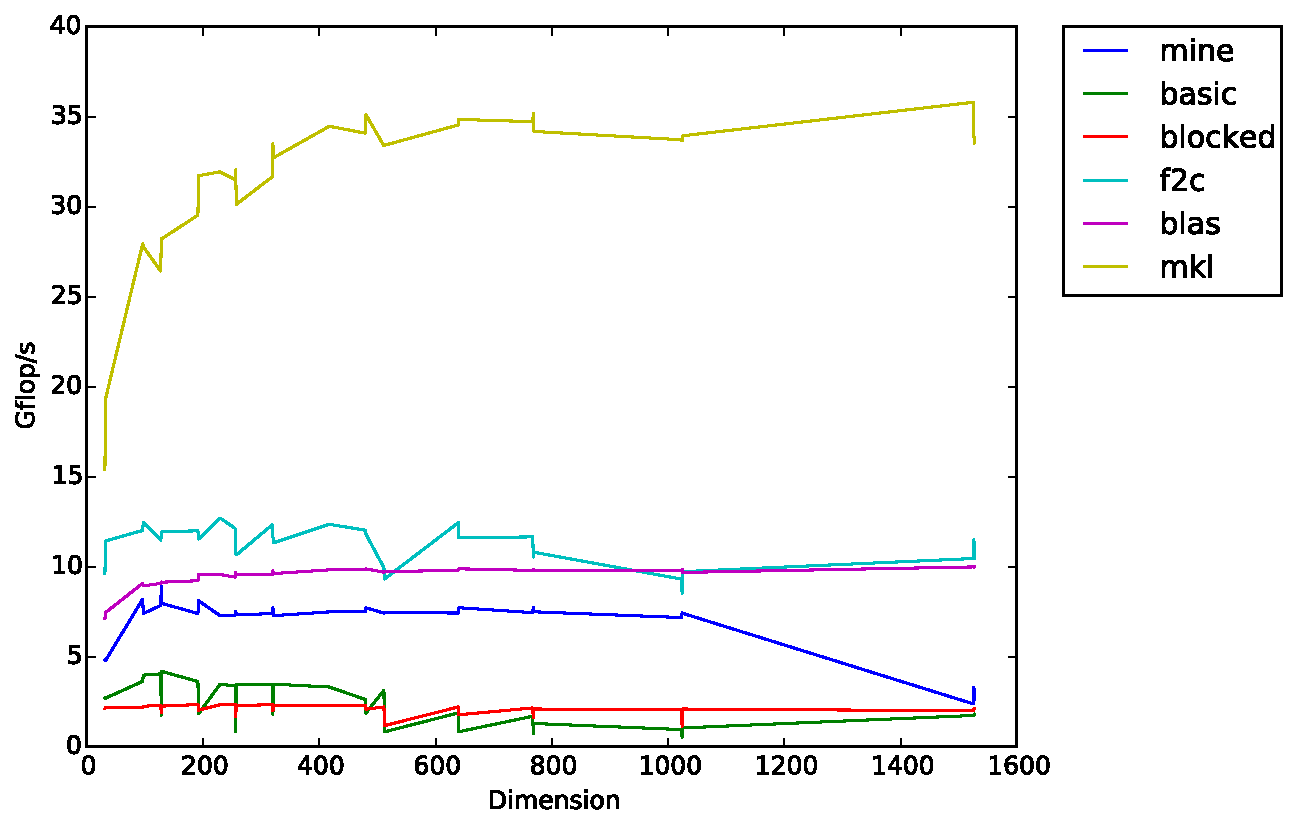
\includegraphics[width=0.8\textwidth]{naive_fortran_opt_flags}
    \caption{Naive Fortran code with optimization flags applied}
\end{figure}

\section*{Analysis:}

Several tuning methods were shown to work fairly well in improving the performance of the matrix-matrix multiplication. The use of optimization flags had by far the largest effect on improving the performance of the code. Next, the blocking worked in that it stabilized the calculations in most cases and resulted in fairly "constant" performance as the size of the matrix increased. However, it can be seen that when comparing Figures 4 and 6 that the blocking method does not perform as well as the non-blocked code. Therefore, what this suggests is that the blocking is still being slowed down by the memory accessing of noncontinuous memory. Better performance could be seen by implementing a multiple blocked strategy that first fits the blocks into L2 cache and then into L1 cache and then finally that can be broken down even more to fit into the registers. Also, once an L1 size block or smaller is taken it could be beneficial then to apply the copy optimization so the data can be aligned with the cache and also be all continuous. Lastly, it can be seen from Figure 3 and 4 that the difference between the C and Fortran code has decreased as more optimizations have been applied to both sets of code.

\section*{References:}

\noindent [1]  https://gcc.gnu.org/onlinedocs/gcc/Optimize-Options.html\#Optimize-Options \\  \\
\noindent [2] https://software.intel.com/en-us/node/579313 \\ \\
\noindent [3] https://software.intel.com/en-us/node/579297 \\ \\
\noindent [4] https://software.intel.com/en-us/node/579324 \\ \\
\noindent [5] https://software.intel.com/en-us/node/579421 \\ \\


\end{document}